\documentclass[10pt]{beamer}
\usetheme{PaloAlto}
\usecolortheme{seahorse}
\setbeamertemplate{navigation symbols}{}
\setbeamertemplate{caption}[numbered]
%general package
%\usepackage[utf8]{inputenc}
\usepackage{array}
\usepackage[english]{babel}
\usepackage{geometry}
\usepackage{tcolorbox}
\usepackage[export]{adjustbox}
\usepackage{graphicx}
\graphicspath{{../img}}

%math package
\usepackage{amsmath}
\usepackage{amsfonts}
%\usepackage{amssymb}
%\usepackage{amsthm}
%\usepackage{slashed}
%\usepackage{tikz-cd}

%font package
%\usepackage{mathrsfs}
%\usepackage{bm}

%misc. package
\usepackage{enumitem}

\DeclareMathOperator{\xd}{\,d\!}
\DeclareMathOperator{\curl}{curl}
\DeclareMathOperator{\dive}{div}
\newcommand{\e}{{\rm e}}
\newcommand{\norm}[1]{\lVert#1\rVert}
\newcommand{\R}{\mathbb R}
\newcommand{\vF}{\mathbf F}
\newcommand{\vv}{\mathbf v}
\newcommand{\inpr}[1]{\left\langle#1\right\rangle}

\author[B.H.]{{\Large MATH211 Calculus III}\\\vspace{6pt}Instructor: Ben Huang}
\date{}
\title[Section 12.3]{Section 12.3 Velocity and Acceleration}
\institute[MU]{
\includegraphics[width = 0.382\textwidth]{MCLogo-Bck.png}}
\logo{
\includegraphics[scale = 0.3]{MCLogo-Bck.png}}

\begin{document}
\frame{\titlepage}

\begin{frame}
\frametitle{Learning objectives}
\noindent
{\bf Learning objectives:} After studying this section, students will be able to
\begin{itemize}[leftmargin=*, label = $\bullet$]
\item find the {\bf displacement}, {\bf velocity} and {\bf acceleration} of an object in motion with given conditions.
\item use vector-valued functions to analyze  {\bf circular motion} and {\bf projectile motion}.
\end{itemize}
\end{frame}

\section{Mechanics}
\begin{frame}
\frametitle{Review of mechanics}
\begin{center}
\begin{tabular}{|c|c|c|}
\hline
&Differentiation&Integration\\
\hline&&\\
Displacement $\mathbf p$&$\mathbf p'=\mathbf v$&\\
(Position)&&\\[3pt]
\hline
&&\\
Velocity $\mathbf v$ &$\mathbf v'=\mathbf a$&$\displaystyle \int_{t_0}^{t_1} \mathbf v(t)\xd t = \mathbf p(t_1)-\mathbf p(t_0)$\\
&&\\
\hline
&&\\
Acceleration $\mathbf a$  &$\mathbf a' = \mathbf{jerk}$ &$\displaystyle \int_{t_0}^{t_1} \mathbf a(t)\xd t = \mathbf v(t_1)-\mathbf v(t_0)$\\
&&\\
\hline
\end{tabular}
\end{center}
Newton's second law: $\mathbf F=m\mathbf a$.
\end{frame}
 
\section{Circular motion}
\begin{frame}
\frametitle{Circular motion}
\centering
\begin{tabular}{cc}
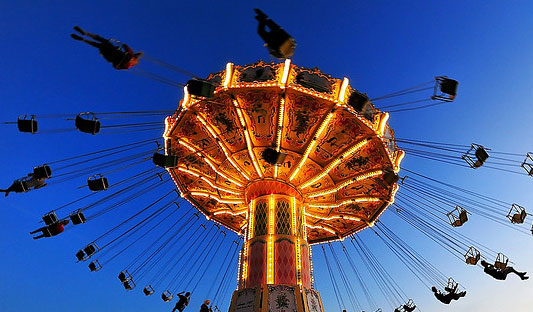
\includegraphics[width=0.3\textwidth]{circular3.jpg}\hspace{2em} &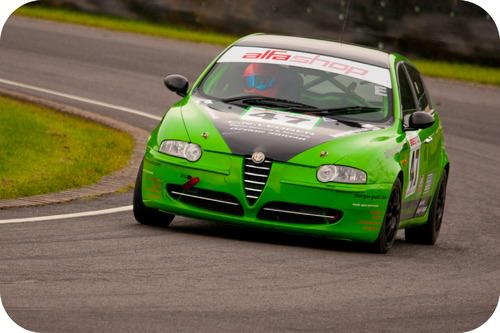
\includegraphics[width=0.3\textwidth]{circular4.jpg}\\
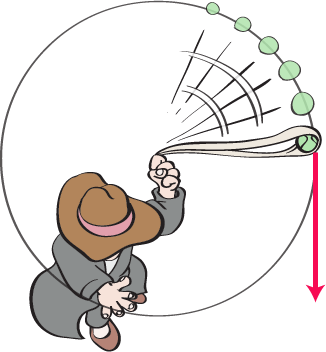
\includegraphics[width=0.3\textwidth]{circular2.png}\hspace{2em} &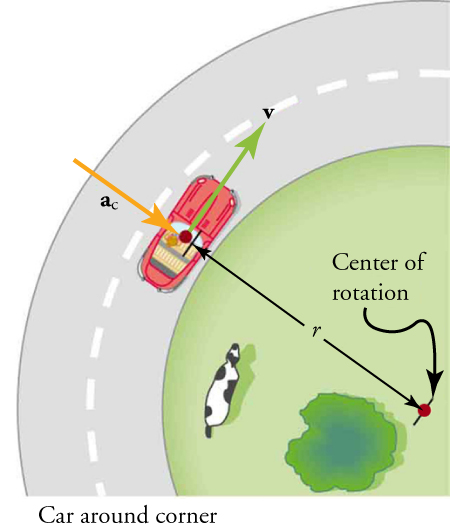
\includegraphics[width=0.3\textwidth]{circular5.jpg}
\end{tabular}\pause

{\bf Circular Motion with Constant Speed:}
 \[ \mathbf r(t) = b\cos(\omega t)\mathbf i + b\sin(\omega t)\mathbf j \]

\end{frame}
 
\section{Projectile motion}
\begin{frame}
\frametitle{Projectile motion}
\begin{figure}
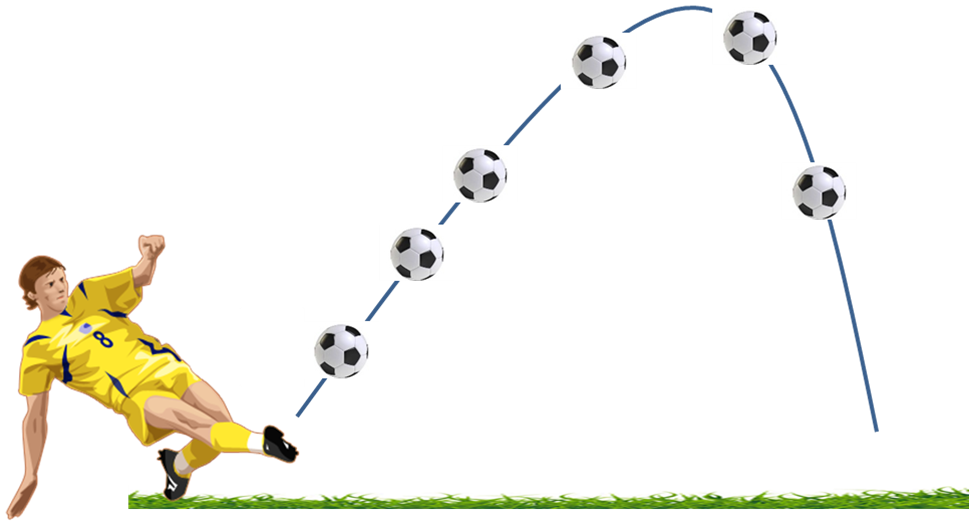
\includegraphics[width=.7\textwidth]{soccer1.png}\\[1em]\pause
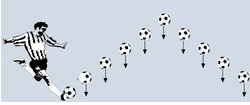
\includegraphics[width=0.6\textwidth]{soccer2.jpg}
\end{figure}
\end{frame}

\begin{frame}
\frametitle{Projectile motion}
\centering
\begin{figure}
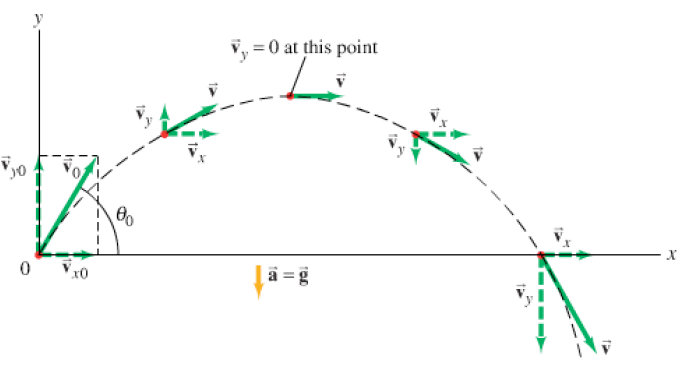
\includegraphics[width=0.75\textwidth]{projectile.png}
\end{figure}\pause
\begin{align*}
&\mathbf a(t)= \mathbf g =-g\mathbf j\\
&\mathbf v(t) = \int_0^t \mathbf a(s)\xd s + \mathbf v_0 = -gt\mathbf j + \mathbf v_0\\
&\mathbf r(t) = \int_0^t \mathbf v(s)\xd s + \mathbf r_0 = -\frac{1}{2}gt^2\mathbf j + \mathbf v_0t + \mathbf r_0
\end{align*}
\end{frame}

\end{document}